\question \textbf{Finite-state machine with 3-grams}
  
Add edges to connect nodes to create an overlap graph that can be used as a 3-gram finite-state machine.

\vspace{0.1 in}

\begin{parts}

%% (a)
  \part List all 3-grams of AAACGGTA.

\begin{solution}[0.5 in]
\begin{verbatim}
AAA, AAC, ACG, CGG, GGT, GTA
\end{verbatim}
\end{solution}

%% (b)
\part Add edges that correspond to the 3-grams of AAACGGTA.

\begin{figure}[H]
      \centering
      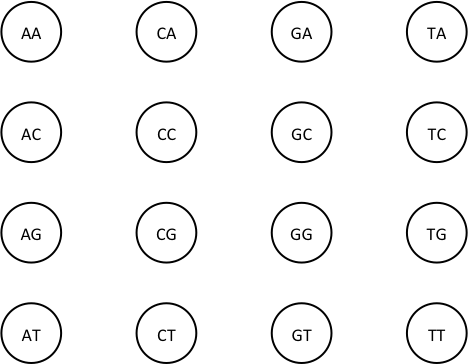
\includegraphics[width=0.4 \textwidth]{fig05/fsm2.png}
\end{figure}

\end{parts}

